\chapter{Conflict Exposure and Competitiveness}
\pubinfo{Francesco Cecchi, Koen Leuveld, and Maarten Voors (2016). Conflict Exposure and Competitiveness: Experimental Evidence from the Football Field in Sierra Leone.\textit{Economic Development and Cultural Change (64-3)}, 405-435}
\label{chap:slfootball}
\renewcommand{\thetable}{\arabic{chapter}.\arabic{table}}


\begin{abstract}
	We use data from a street football tournament and a series of lab-in-field experiments in post-conflict Sierra Leone to examine the impact of exposure to conflict violence on competitive behavior. We find that football players that experienced more intense exposure to violence are more likely to get a foul card during a game. In the lab we find that these individuals are significantly less risk averse and more altruistic towards their in-group (teammates). We then isolate competitiveness from aggressiveness and find that conflict exposure increases the willingness to compete towards the out-group. These results are in line with theory highlighting the role of inter-group conflict in increasing in-group cooperation while exacerbating out-group antagonism. Next to other-regarding preferences and risk propensity, changes in individual preferences for competition may impact long-run development trajectories and post-conflict recovery.
\end{abstract}


\section{Introduction}
More than two-thirds of African nations have experienced civil war during the past decades \citep{Themner2014}. Research in the consequences of these conflicts documents the persistent effect of violence on education \citep{Lai2007a,Chamarbagwala2011},health and disability \citep{Ghobarah2003,Iqbal2006a,Iqbal2010a}, food security and poverty \citep{Gates2012} and the working of societies as a whole. The impacts on institutions, individual behavior and preferences are less well understood \citep{Blattman2010b}. There is a small but growing body of literature examining these impacts, predominantly highlighting changes in social and political preferences, such as participation in local collective action, voting and sharing both within and across communities. Evolutionary theory highlights the role of inter-group conflict in shaping pro-egalitarian parochial preferences – increasing in-group cooperation while exacerbating out-group antagonism \cite{Bowles2006b,Bernhard2006b,Choi2007a}. At shorter time-scales this theory has been corroborated with respect to increased in-group cooperation after civil war \cite{Bellows2009b,Voors2012,Gilligan2014,Bauer2014}, and increased out-group antagonism \citep{Miguel2011b}.

Increased out-group antagonism may impact the aggressiveness of individuals \citep{Miguel2011b}, but it may also affect their willingness to compete. Taste for competition is an important non-cognitive determinant of human capital indicators, such as adult economic achievements and productivity \citep{Niederle2007}. If less competitive people shy away from direct competition \citep{Bartling2012}, non-first-best contenders have a higher chance of winning a contest, affecting allocative efficiency \citep{Eriksson2009a}. For this reason, “competitions and the right dose of competitiveness significantly determine not only the future of the individual but even the evolution of the whole species” \citep{Leibbrandt2013}. Yet, individual variations in competitiveness need not to be solely explained by genetic endowments and long-run evolution. They may be the result of exposure to different environments and pressures. \cite{Leibbrandt2013} compare individualistic and collectivistic societies, and show that life experiences may alter individual tastes for competition.  In conjunction with altered preferences for local collective action and trade-offs over risk and time, shifts in competitiveness may be a crucial determinant of regional post-war political and economic recovery and development. 

This paper seeks to connect and contribute to two literatures: that on the determinants of competitiveness and on the impact of civil war (which we discuss below). Several authors argue that conflict exposure during childhood affects beliefs and behavior later in life \citep[see][for a review]{Adhvaryu2013}. Using data from a football tournament in Sierra Leone, we assess the impact of war-related violence on preferences of local youth. We carefully record the details of each match and player. After the game, we invite players to participate in a series of lab-in-field experiments and a short survey. We measure preferences towards teammates and opponents, making use of the bi-lateral antagonism and group dynamics generated by sport itself \citep[see][]{Weinstein1995a,Duggan2002a,Garicano2006,Miguel2011b}. We find that individuals who experienced more intense conflict-related violence during childhood are more likely to receive a foul card during a football game, are less risk averse and more altruistic towards their in-group, but not towards the out-group. Next, we test willingness to compete through an effort game that disentangles competitiveness from aggressiveness. Out-group competitiveness appears to be exacerbated by violent conflict: conflict exposed subjects are on average 51\% more likely to enter a competition against an out-group than the non-exposed. 

Obviously, it is challenging to identify the exact mechanisms through which conflict affects behavior. We argue that our results are consistent with a perspective on how conflict changes preferences and beliefs. To probe the robustness of our results we run several checks. First, we investigate self-selection into violence and find little evidence of it—consistent with literature on the Sierra Leonean civil war. Next, we show that age-group fixed effects (plausibly correlated with war exposure) do not alter our main result. Also, we probe whether our results are driven by temporary migration: our main coefficient remains stable and is not significantly different across war time migration destinations. In addition, our main result is robust to the introduction of forced displacement as an additional source of war-related trauma, as well as to football match and team fixed effects, and clustering standard errors at the football team level. Finally, willingness to compete may also be a function of risk preferences, expected relative performance, and actual skills. We show that our result maintains when controlling for these covariates both separately and jointly.

The study is organized as follows. Section \ref{sec:slfootball:litreview} discusses literature on conflict and preferences and on the determinants of competitiveness and presents our key hypothesis. Section \ref{sec:slf:background} presents the context and background of civil war in Sierra Leone and of our study area in particular. Section \ref{sec:slf:data} introduces the field and lab experimental data, and outlines the experimental design and data. Section \ref{sec:slf:identification} discusses our identification strategy and Section \ref{sec:slf:results} contains our results. Section \ref{sec:slf:discussion} offers a discussion and conclusion.

\section{Conflict, preferences and competition}
\label{sec:slfootball:litreview}
Competitiveness is a key determinant of individual economic achievements and productivity \citep{Niederle2007}. There are significant differences in willingness to compete both within and across societies \citep{Leibbrandt2013}. These differences can are attributed to variations in genetic endowments, abilities and preferences \citep{Niederle2007,Gneezy2009} as well as individual exposure to various environmental pressures and life events \citep{Roth1995}. Most empirical studies on the origins and consequences of competitiveness use data from laboratory experiments. Using effort games, behavioral economists document that when the type of payment is exogenously imposed on subjects, competitive tournaments reveal a much larger variance of effort than equivalent piece-rate schemes \citep{Dijk2001,Harbring2003a}. This in turn reduces their overall efficiency \citep{Eriksson2009a}. Such an unexpected finding may be driven by the unwillingness of some people to enter competition. In fact, \cite{Eriksson2009a} show that allowing for self-selection into a competitive tournament results in higher average effort rates and lower between-subject variance for subjects choosing to compete. Competitive environments are thus more efficient than non-competitive ones only if populated by a sufficient share of agents willing to compete.

While a complete insight is lacking, literature has highlighted several individual and behavioral determinants of competitiveness. For example, \cite{Niederle2007} find important differences with respect to gender and performance expectations. \cite{Bartling2009b} find that overconfident, skilled and risk prone subjects are more likely to join a contest, while inequality-averse subjects less. \cite{Leibbrandt2013} find that fishermen from individualistic societies are far more competitive than those from neighboring collectivistic societies, and that this difference emerges with time. Individuals shape their preferences mostly during childhood \citep{Benenson2007,Fehr2008}, and continue to develop them till early adulthood \citep{Sutter2007a}. Intense shocks during childhood should thus alter individual preferences for competition. Yet, the role of early life events such as exposure to conflict as a determinant of competitiveness is still ill-understood.
Research into conflict induced changes in behavior is equally limited but growing \citep{Blattman2010b}.\footnote{Psychological literature documents the relationship between war exposure and trauma, focusing mostly on post-traumatic stress disorder (PTSD), anger and anxiety. \citet{Macksoud1996a} examine the relation between war traumas and psychosocial development, finding that the number of war traumas experienced by a child was positively related to Post Traumatic Stress Disorder (PTSD) symptoms and differentially related to other behavioural outcomes. \citet{Smith2002} and \citet{Layne2010} identify similar attitudinal outcomes among conflict exposed children in Bosnia, while \citet{Dyregrov2002} find highly time-persistent intrusive and avoidance reactions among Iraqi children exposed to a deadly aerial bombing. Other studies explore instead positive responses to trauma––often referred to as ``post-traumatic growth'' \citep{Tedeschi1996,Powell2003,Staub2008,Vollhardt2009}.} A key research line focusses on the impacts on pro-social preferences. An emerging insight points to the boundary between in-groups relative to out-groups in shaping post conflict preferences: intra-community violence appears to decrease within community social cohesion whereas inter-community conflict increases it. This mirrors contributions in evolutionary theory, which predicts how inter-group conflict shapes parochial preferences—increasing in-group cooperation while exacerbating out-group antagonism \citep{Bowles2006b,Bernhard2006b,Choi2007a}. For example, \cite{CassarAlessandra} find that intra-community violence in Tajikistan undermined social cohesion and in-village trust \citep[see also][]{Rohner2013}. On the other hand, \cite{Bellows2009b} find that Sierra Leoneans whose households directly experienced more intense violence by the RUF are more likely to attend community meetings, join local political and community groups, and vote. \cite{Blattman2009a} finds that experiencing abduction and violence increased political engagement, voting and community leadership among ex-combatants in Northern Uganda. \cite{Blattman2010b} present a survey of literature on civil war and argue that the existing literature omits advances in behavioral economics, and advocate micro-level analysis and case studies as crucial to understand war’s causes, conduct, and consequences, in particular in the behavioral and institutional domain.  

In recent years, a number of studies have used lab-in-field experiments to gauge the consequences of civil wars. \cite{Voors2012} show that individuals exposed to violence display more altruistic behavior towards their neighbors, are more risk-seeking, and have higher discount rates. \cite{Gilligan2014} show that communities that suffered war-related violence during Nepal's ten-year civil war exhibit significantly greater levels of altruistic giving, public good contributions, investment in trust-based transactions, and willingness to reciprocate trust-based investments. \cite{Bauer2014} investigate how conflict experiences shape the beliefs and preferences of youth. They present two case studies – one in Georgia and one in Sierra Leone – indicating that experiencing inter-group conflict during childhood and adolescence increases egalitarian motivations toward the in-group, but not the out-group. The only work that explicitly investigates behavioral changes in out-group antagonism is \cite{Miguel2011b}, who examine the consequences of civil war on aggressiveness of players in European football leagues. They find that the number of years the home country of a player has been in violent conflict before the player reaches the age of eighteen is strongly and positively related to the amount of foul cards received. 
We build on work by \cite{Miguel2011b}, and combine data from a field setting – the football tournament – and lab-in-the-field experiments. After providing confirmatory evidence of increased aggressiveness and increased parochial altruism, we test willingness to compete through a competitiveness game that disentangles competitiveness from aggressiveness—i.e. a player’s choice to compete may only affect his own payoff, not that of other  players. While the role of conflict exposure in shaping social preferences has been explored in several experimental settings, to our knowledge this is the first work attempting to investigate its effect on competitiveness.

\section{Background: the Sierra Leone civil war}
\label{sec:slf:background}
We use data from a sample of respondents in Kenema, a regional town in Eastern Sierra Leone. Sierra Leone is amongst the poorest countries in the world recovering from an eleven years long civil war (1992-2001). At its start, a small group of rebels entered the East of the country. They found fertile ground for popular grief and discontent towards “a decayed neo-patrimonial one-party regime” \citep{Richards1999} and were nurtured by Sierra Leone’s diamond wealth \citep{Keen2005a}. It was the start of a country-wide civil war that cost over 50,000 lives, leaving many civilians amputated and abused, and hundreds of thousands temporarily displaced \citep{HumanRightsWatch1999a,Doucet2012a}.

Kenema is the gateway to the eastern provinces and forested Liberia border area. The district saw many conflict events throughout the war; in fact the “Zogoda”, RUF’s headquarters, was only about 30 km from Kenema \citep{Peters2011}. While there were many parties involved in violence in the war, most was committed by the RUF \citep{Conibere2004}.  The conflict in Kenema can be separated in three phases: the initial incursion and consolidation by the RUF (1991-1993), clashes between Civil Defence Forces (CDF, or Kamajors) and the RUF , up to 1997, and a final phase which saw widespread intervention by ECOMOG, from 1997 – 2000. During all phases of the war, most violence was motivated either to cause fear and panic or to obtain supplies by the belligerent parties, both resulting in indiscriminate violence against civilians. During so-called “food finding missions” houses were looted and burned \citep[for a broader discussion on such tactics, refer to Kalyvas ][]{Kalyvas2006}. Civilians were regularly captured to work in mines, raped, or mutilated. A report submitted to the Special Court for Sierra Leone \citep{Smith2004a} describes the events in detail. During a typical attack “RUF forces fired indiscriminately at civilians, who were running here and there, dazed and confused, killing dozens. Many houses were burnt and massive looting was carried out, with people of the town being forced to carry the stolen property” \citep[p.~303]{Smith2004a}. The most notable direct attack by RUF forces took place on Christmas Day in 1994. The attack, which lasted several days, resulted in the deaths and abduction of hundreds of civilians. Later in 1997, when the RUF briefly ruled the town, “girls were raped, houses were looted continuously and civilians were harassed for food and other items” \citep[p.~318]{Smith2004a}. These events reflect the national patterns of conflict, where most violence was not motivated by religious or ethnic cleavages \citep[see][]{Bellows2009b}, and no ethnic group was disproportionally targeted by rebels \citep{Conibere2004,Humphreys2006}.\footnote{See Section \ref{sec:slf:identification} for a further discussion and analysis.} 
Most of our respondents lived in Kenema during the conflict. Figure \ref{fig:slf:conflictexposure} shows the distribution over time of conflict related events, war exposure and conflict induced displacements, of our sample. As a confirmatory exercise we have plotted the recorded violent events in Kenema from the SLL-LED dataset \citep{Bruijne2014} in the figure as well. Two peaks, in 1994 and 1997-1998 overlap with exposure and displacement events in our sample. Over 82\% of our respondents were (temporarily) displaced at least one time during the conflict. This is comparable to the nationally representative wartime displacement rates in the 2007 Institutional Reform and Capacity Building Project dataset  used in \cite{Bellows2009b}. While some of our respondents moved to places out of Sierra Leone (neighboring Guinea and Liberia), most displacements where within Kenema district (51.1\%) or adjacent districts (11.9\%). 

\begin{figure}[p!]
	\begin{center}
	  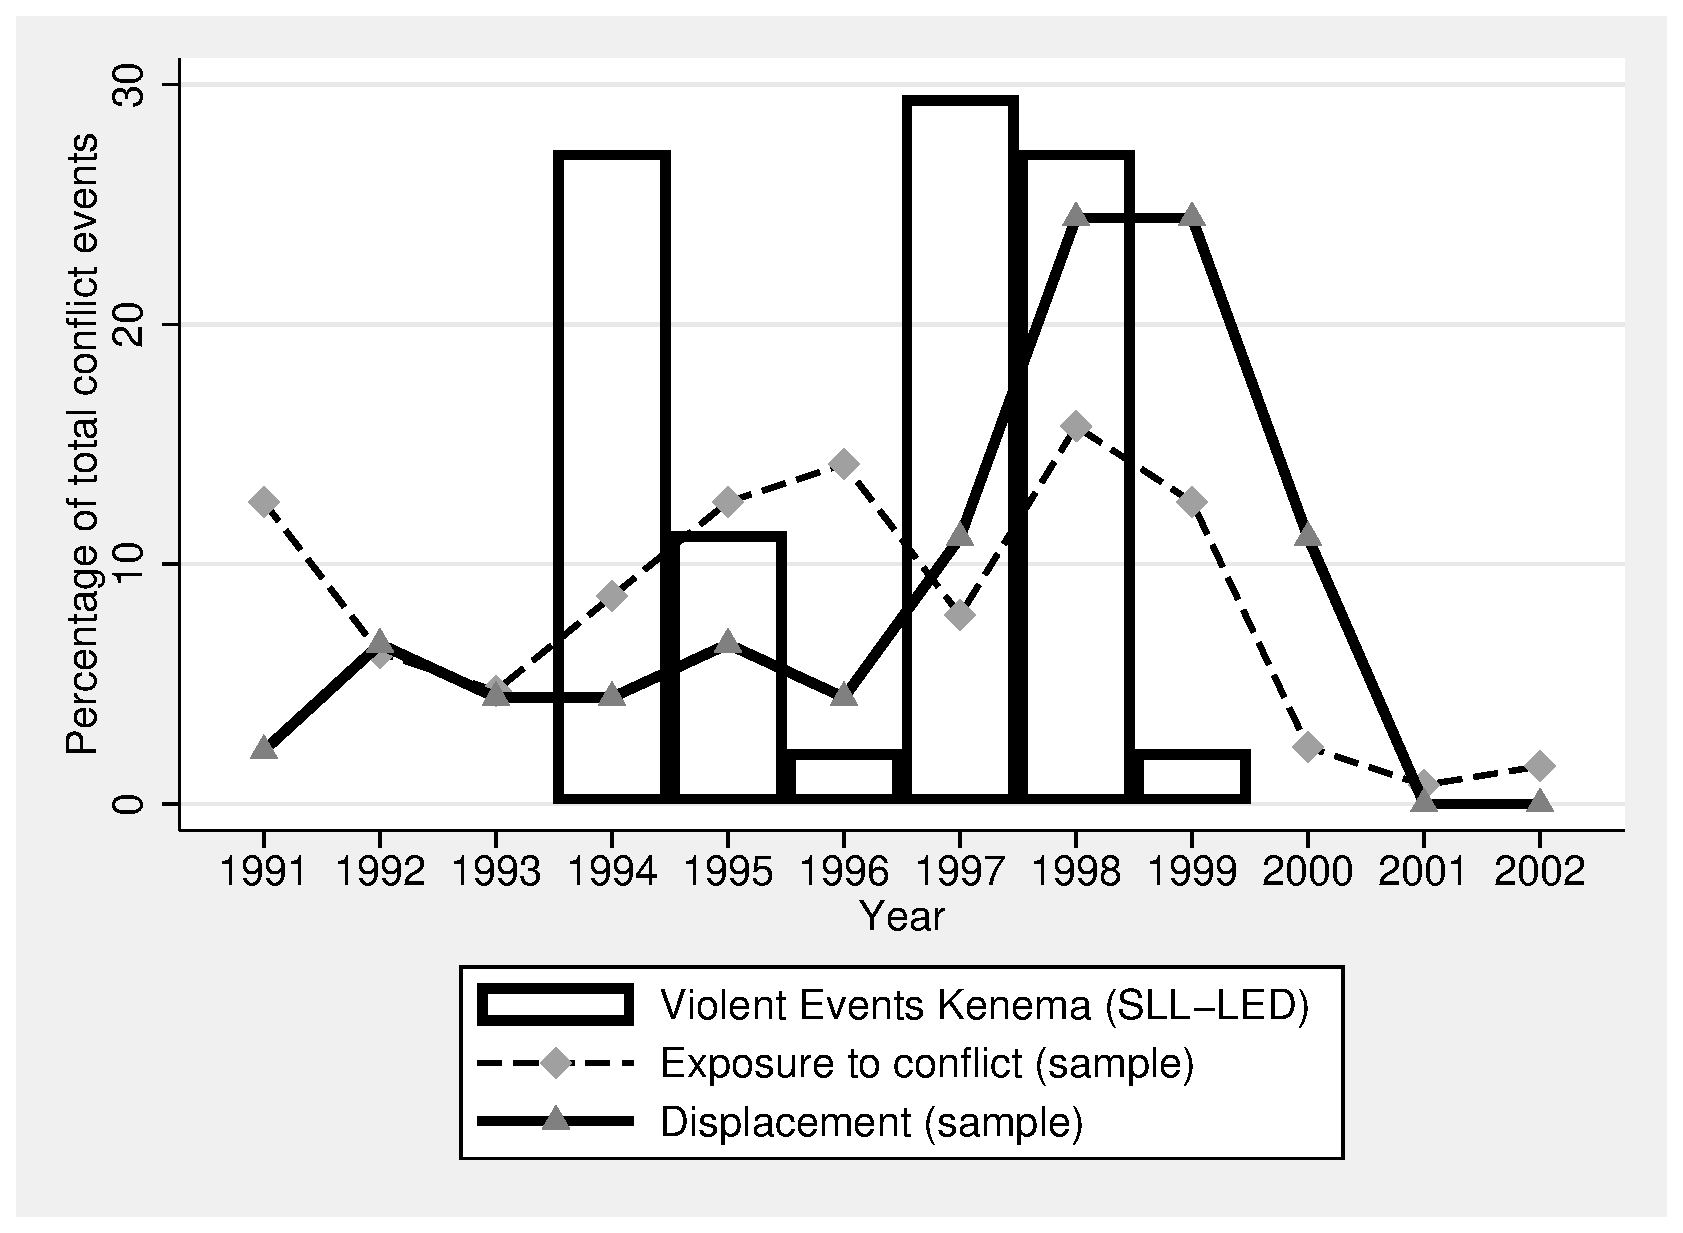
\includegraphics[width=0.7\linewidth]{"chapters/slfootball/figures/f1_violent_events.eps"}
	  \caption{Exposure to conflict, and displacement in our sample over time, combined with SLL-LED attacks events in Kenema District over the same time period.} \label{fig:slf:conflictexposure}
	  \subcaption*{\textit{Notes:} distribution of SLL-LED events in Kenema \citep{Bruijne2014}, conflict events reported by participants and displacement events reported by participants over the course of the war in Sierra Leone. All data is presented as column totals, so about 25\% of all displacement events took place in 1998.}
	\end{center}
\end{figure}

Disarmament started at the end of 2001 and President Kabbah declared the war over in January 2002 \cite{Peters2011}. RUF and other armed groups were disarmed, demobilized and reintegrated in society. At present violence and intimidation have disappeared from Sierra Leone and the country has now known several years of peace. While the country still ranks low on close to all development indicators, the local economy is improving each year––the 2013 GDP growth rate was close to 13\%.

\pagebreak
\section{Data and experimental design}
\label{sec:slf:data}
Our data was collected during a youth street football tournament organized in Kenema. The tournament spanned several weeks between November and December 2010. For the tournament, streets within the city each assembled in a team. Matches were centrally organized and a substantial cash reward awaited the winner. Team identity was strong and the players took pride in defending their street. Referees oversaw adherence to rules and distributed yellow and red cards in response to minor and major fouls.\footnote{Two referees oversaw all the football games. The referees were semi-professional and provided by the organisation of the tournament (a youth association in Kenema). One could worry that the referees systematically favoured one team over the other based on its composition. We have no reason to believe this is the case, but cannot rule this out completely. Unfortunately, we did not collect information about the referee’s background, ethnic group, and individual characteristics.}  We carefully recorded details of the matches and players of the performance of 14 teams and 162 players.  Table \ref{tab:slf:summstats} presents the descriptive statistics (see Appendix I for variable definitions). A total of 47 yellow and 3 red cards were given, involving 20\% of the players. After each football match, we invited players to participate in a survey and a series of lab-in-field experiments. Our close collaboration with tournament organizers and team managers effectively cancelled attrition. 

%tables
%\begin{adjustbox}{totalheight=\textheight-2\baselineskip}
\begin{center}
	\begin{threeparttable}[p!]
	
		\caption{Descriptive Statistics}
		\label{tab:slf:summstats}
		\renewcommand{\arraystretch}{0.6}
		% \tiny 
		% \scriptsize
		%\footnotesize
		% \small
		% \normalsize
		{
\def\sym#1{\ifmmode^{#1}\else\(^{#1}\)\fi}
\begin{tabular}{l*{1}{ccccc}}
\hline\hline
                    &\multicolumn{5}{c}{}                                            \\
                    &       count&        mean&          sd&         min&         max\\
\hline
Exposure to conflict&         162&        0.57&        0.26&        0.00&        1.00\\
Parent fought in war&         162&        0.12&        0.33&        0.00&        1.00\\
ind\_age             &         162&        1.72&        1.01&        1.00&        5.00\\
ind\_edu             &         162&        2.54&        0.61&        1.00&        3.00\\
Meals per day       &         162&        2.44&        0.63&        1.00&        3.00\\
Muslim              &         162&        0.79&        0.41&        0.00&        1.00\\
Mende               &         162&        0.54&        0.50&        0.00&        1.00\\
ind\_alwaysken       &         162&        0.52&        0.50&        0.00&        1.00\\
Foul card           &         162&        0.20&        0.40&        0.00&        1.00\\
Played whole game   &         162&        0.46&        0.50&        0.00&        1.00\\
Self-declared skills&         162&        0.86&        0.23&        0.00&        1.00\\
Scored              &         162&        0.17&        0.38&        0.00&        1.00\\
Won the football game&         162&        0.42&        0.50&        0.00&        1.00\\
Left footed         &         162&        0.19&        0.39&        0.00&        1.00\\
Risk Preferences    &         162&        0.00&        1.00&       -1.56&        1.19\\
0 life\_dict         &         162&       -0.27&        1.09&       -3.43&        2.39\\
1 life\_dict         &         162&        0.27&        0.81&       -2.70&        3.84\\
Outgroup Tournament &          70&        0.43&        0.50&        0.00&        1.00\\
Ingroup Tournament  &          92&        0.41&        0.50&        0.00&        1.00\\
Expected performance&         162&        0.91&        0.13&        0.60&        1.00\\
Balls on target     &         162&        6.27&        1.82&        1.00&       10.00\\
\hline\hline
\end{tabular}
}

		\begin{tablenotes}
			\footnotesize
			\item \textit{Notes:} See Appendix I for variable definitions.
		\end{tablenotes}
	
	\end{threeparttable}
\end{center}
%\end{adjustbox}

Our respondents are young males, between 14 and 31 years old (see Figure \ref{fig:slf:ageconflict}A). They are predominantly Muslim, and of the Mende tribe and 50\% are enrolled in senior secondary education. We identify a series of plausible non-experimental proxies of sportive ability, which may influence the willingness to compete and to receive a foul card. Substitutes could enter and exit at any time of the match, with no limit with respect to the number of substitutions. Therefore, whether a player had not been substituted during the entire duration of the match (46\%) may be seen as a good approximation of relatively greater football skills, most likely correlated to general sportive ability. In addition, we ask our respondents to rate their own level of skills compared with their teammates. We create an index ranging from 0 (self-declared least skilled) to 1 (self-declared most skilled). While we could not record the positioning of players on the football field due to the high fluidity of play, we also recorded which players scored a goal. Finally, we recorded which team won the football game,\footnote{The decision of entering the competition may be influenced by the expected ability of the counterpart. Participants could only estimate team-level ability at the team level, as counterparts are anonymous, which is proxied by winning the football game. Also, winning the football game may have implications for the morale and overconfidence of participants.}  and if the participant is left or right footed.\footnote{Psychological literature highlights correlations between handedness and several non-cognitive dimensions \citep{Goldberg1994} as well as cognitive skills \citep{Sanders1982,Faurie2006}. More recently, handedness has been placed in correlation with economic outcomes \citep{Denny2007} and competitiveness \citep{Hoffman2010}. Less attention has been devoted specifically to footedness. However, footedness is strongly correlated with handedness – especially for right-handers \citep{Peters1979} – and \citet{Elias1998} find it to be a more accurate predictor than handedness of emotional lateralization.}

\begin{figure}
	\begin{centering}
	  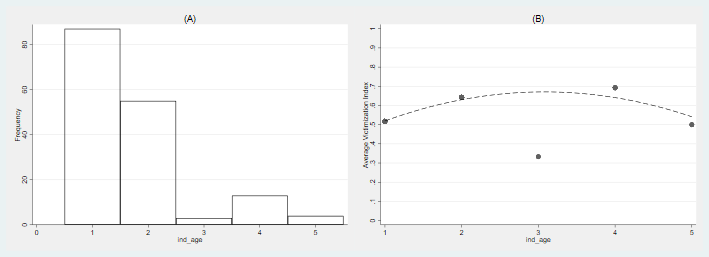
\includegraphics[width=\linewidth]{"chapters/slfootball/figures/f2_agefreq_agewe.eps"}
	  \caption{Age in sample and exposure to conflict}
	  \label{fig:slf:ageconflict}
	  \subcaption*{\textit{Notes:} panel A shows the distribution of age in our sample. Panel B shows the relationship between age and victimization index.}
	 \end{centering}
\end{figure}


To measure exposure to conflict-related violence we ask respondents about a range of war related events, covering information on personal injury, seeing injured people, seeing and hearing combat.\footnote{In a robustness check we include displacement as an additional element of the victimization index. As 82\% of our sample was temporarily displaced at least once during the conflict, this brings average victimisation up to 0.63 (0.24). See section \ref{sec:slf:results} for the implications of this change for our results.} Following \cite{Bellows2009b}, we create a victimization index using the average of positive responses to these violence related questions. On average, our respondents experienced 57\% of such events.\footnote{This statistic is similar to what \citet{Bellows2009b} find in their study. Note that, as our measure of war exposure is self-reported, one may worry that types of respondents have a different propensity to report on war time events. If this is correlated with our outcome variables, then our estimates are biased. While we cannot exclude such possibility, our data show consistent patterns results for those reporting high and low levels of conflict exposure reducing concerns over bias in reporting.}  Figure \ref{fig:slf:ageconflict}B shows the average conflict exposure by age in our sample. Younger generations are relatively less victimized, but overall victimization follows a rather clear quadratic trend across age groups (a more detailed discussion on this can be found in Section \ref{sec:slf:identification}).

We implement a range of lab-in-field experiments. We measure willingness to self-select into competitive environments using an effort game, based on \cite{Niederle2007} and \cite{Bartling2009b}. Respondents are invited to participate in a game where they throw a football into a standard sized basket secured to the floor, from a distance of four meters. They choose whether to play individually – at a piece rate payment scheme of 500 Leones per ball on target – or to enter a competition against an anonymous counterpart. In the competition, the respondent wins 1500 Leones for every ball on target if the total number of hits is higher than the counterpart––zero if lower.\footnote{4400 Leones were about 1 USD at the time of data collection.}   In case of a draw with the counterpart the respondent receives 500 Leones per ball on target. It is possible for one player to enter the competition even if the counterpart does not, and vice versa. As a result, the payout of one player is determined only by his choice to compete and by the number of balls on target relative to the anonymous counterpart.\footnote{For example, even if player 1 decides to not compete, player 2 would get zero pay-out in case player 2 decides to compete and scores less than player 1. Oppositely, even if player 1 decides to compete, player 2 would not lose if he decides not to compete.}  In other words, participants cannot influence or hurt their opponents’ utility and earnings by choosing to enter the competition—but only by being better, regardless of their choice to compete or not. This setup allows us to disentangle willingness to compete from aggressiveness, as the decision to compete or not taken by each participant only affects their own private outcome, and not that of the counterpart. Respondents are randomly divided into two groups: one group plays against an anonymous player of the opponent team (out-group) and another against an anonymous player of their own team (in-group). 42\% of the respondents chose to participate in the tournament. Figure \ref{fig:slf:ballshit} shows the distribution of balls on target and relative frequency across groups. On average, respondents scored 6.27 hits (out of 10 tries), with a standard deviation of 1.82.\footnote{To control for expected performance in a sensitivity analysis, we ask respondents to assess their expected performance prior to playing the game. We create an index ranging from 0 (self-declared worst expected performance) to 1 (self-declared best expected performance).}  

\begin{figure}
	\begin{centering}
		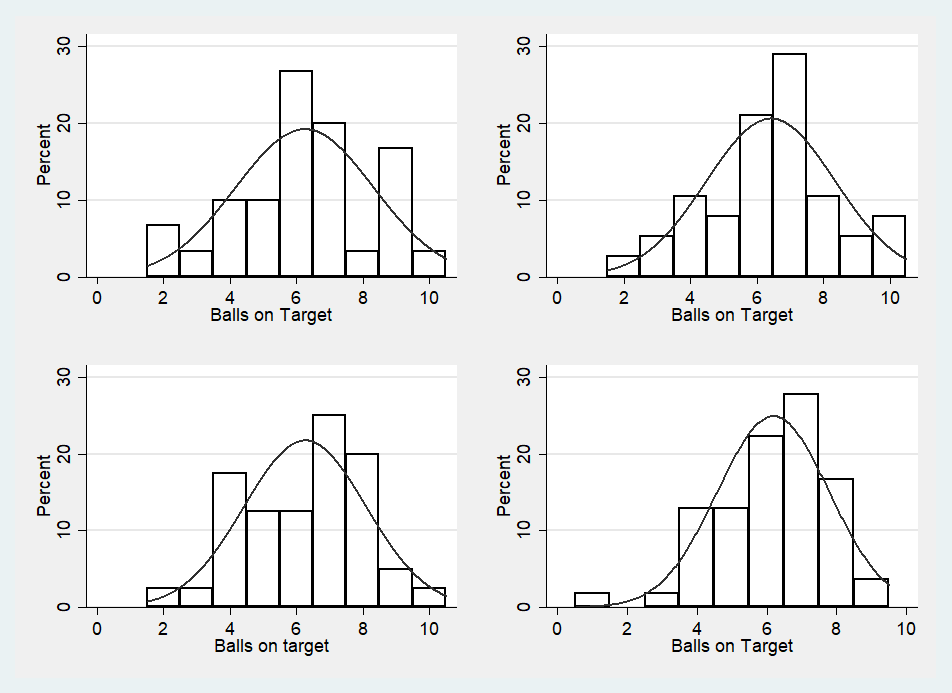
\includegraphics[width=0.6\linewidth]{"chapters/slfootball/figures/f3_ballshit.eps"}
		\caption{Balls hit in the effort game}
		\label{fig:slf:ballshit}
		\subcaption*{\textit{Notes:} distribution of number of balls hit for four subsamples: Panel A: Out-group, opted for tournament; Panel B: In-group opted for tournament; C: Out-group, did not opt for tournament; D: In-group, did not opt for tournament }
  \end{centering}
\end{figure}

To measure risk preferences, we use a simple dichotomous choice game based on \cite{Harbaugh2002a}. In this risk game subjects are required to choose several times between receiving an amount of money for certain and playing a simple gamble. Six choice sets are presented; each time we ask whether the respondent prefers (1) to toss a coin and make the chance of winning 3000 Leones or zero (if tails), or (2) not toss a coin and win an amount of money for certain, growing in each choice set, from 100 Leones to 2500 Leones. The expected value of the gamble is thus kept constant, while the certain option increases progressively: the point of switch from the gamble to the certain option is used to determine the risk preferences of the respondent \citep[see][]{Harbaugh2002a} –– the later the switch, the less risk-averse (Table \ref{tab:sl:riskchoice}). We then standardize the resulting discrete variable to improve the interpretability of the findings.

\begin{table}
	\centering
	\begin{threeparttable}
	\singlespacing
	\caption{Risk Propensity Game Choice Sets}
	\begin{tabular}{cccc}
		\toprule
		      & \multicolumn{2}{c}{Coin Toss} &  \\
		Choice set & If heads & If tails & For certain \\
		\midrule
		1    & 3000  & 0     & 100 \\
		2    & 3000  & 0     & 500 \\
		3    & 3000  & 0     & 1000 \\
		4    & 3000  & 0     & 1500 \\
		5    & 3000  & 0     & 2000 \\
		6    & 3000  & 0     & 2500 \\
		\bottomrule
	\end{tabular}%
	\begin{tablenotes}
		\item \textit{Notes:} monetary amounts are reported in Leones. The exchange rate at the time of data collection was about 4400 Leones to 1 USD.
		\item
	\end{tablenotes}
	\label{tab:sl:riskchoice}%
	\end{threeparttable}%
\end{table}

To gauge other-regarding preferences we use a simple non-strategic dictator game. Each participant made two choices about how to allocate a given endowment, once paired with a teammate and once with an opponent, in random order. Players received 1000 Leones and were told these were theirs to keep at the end of the experiment. Alternatively, they could donate any 50 Leones portion of it to an anonymous counterpart. To avoid income effects potentially confounding our results, participants were notified that their final pay-off would be determined by the outcome of one randomly selected game they played, plus a possible donation from either a teammate or an opponent. Also in this case, we standardize out-group and in-group donations for the sake of interpretability.

\section{Identification and empirical strategy}
\label{sec:slf:identification}

Our empirical strategy relies on local comparisons across war and non-war exposed subjects. The key identifying assumption is that exposure to violence was exogenous with respect to individual characteristics. This assumption may be violated in the presence of systematic targeting by belligerents along some individual dimension––i.e. religion, ethnic group, etc. While undoubtedly some elements of violence were targeted, most violence in Sierra Leone was essentially a random process \citep{Conibere2004,Humphreys2006,Bellows2009b}). To test these assumptions on our own sample of respondents, below we regress war exposure on a set of variables capturing individual characteristics.\footnote{Our sample does not include traditional authority households – significantly more likely to experience violence during the civil war according to \citet{Bellows2009b}. We do have information on participation in civic defence forces (CDF). Individuals whose parents participated in CDFs or independently fought during the civil war may have experienced more violence. In particular, if those individuals were more competitive, and competitive behaviour is correlated across generations, the main coefficient might reflect selection rather than the treatment effect of exposure to violence. Columns 3 and 4 of Table \ref{tab:slf:conflictexposure} show how there is no evidence of a significant self-selection effect into war related violence for the children of combatants. Also, Column 4 highlights how war exposure does not significantly correlate with any of the proxies for athletic ability identified during the football game.} We find no evidence of selective violence, except for age (and age squared); responding to intuition, older participants faced a higher probability of war exposure (Table \ref{tab:slf:conflictexposure} and Figure \ref{fig:slf:ageconflict}B).\footnote{Of course, there may be selection bias due to unobservable characteristics not captured in our data, for example ethnic or political cleavages may make people more prone to be targeted. If political cleavages are related to competitive behavior, then this will bias our estimates. While we cannot rule out such hypotheses entirely, the nature of violence in Sierra Leone does not indicate such cleavages matter for victimization, and the results of Table \ref{tab:slf:conflictexposure} seem to indicate homogeneous victimization across ethic groups \citep[see also][]{Bellows2009b}.}

\begin{table}[p!]
	\centering
	\begin{threeparttable}[p!]
		\caption{Exposure to Conflict}
		\singlespacing
		%\setlength\extrarowheight{-10pt}
		%\renewcommand{\arraystretch}{0.6}
		% \tiny 
		% \scriptsize
		%\footnotesize
		\small
		% \normalsize
		\label{tab:slf:conflictexposure}
		{
\def\sym#1{\ifmmode^{#1}\else\(^{#1}\)\fi}
\begin{tabular}{l*{4}{c}}
\hline\hline
                    &\multicolumn{1}{c}{(1)}         &\multicolumn{1}{c}{(2)}         &\multicolumn{1}{c}{(3)}         &\multicolumn{1}{c}{(4)}         \\
\hline
Age                 &       0.196\sym{***}&       0.172\sym{***}&       0.193\sym{***}&       0.160\sym{***}\\
                    &    (0.0528)         &    (0.0558)         &    (0.0529)         &    (0.0564)         \\
[1em]
Age squared         &    -0.00407\sym{***}&    -0.00358\sym{***}&    -0.00400\sym{***}&    -0.00326\sym{**} \\
                    &   (0.00121)         &   (0.00127)         &   (0.00122)         &   (0.00128)         \\
[1em]
Muslim              &                     &    0.000515         &                     &      0.0224         \\
                    &                     &    (0.0464)         &                     &    (0.0523)         \\
[1em]
Mende               &                     &      0.0252         &                     &      0.0327         \\
                    &                     &    (0.0607)         &                     &    (0.0648)         \\
[1em]
Fula                &                     &     -0.0952         &                     &     -0.0727         \\
                    &                     &    (0.0843)         &                     &    (0.0905)         \\
[1em]
Mandingo            &                     &     -0.0859         &                     &     -0.0662         \\
                    &                     &    (0.0893)         &                     &    (0.0978)         \\
[1em]
Temne               &                     &     -0.0555         &                     &     -0.0677         \\
                    &                     &    (0.0955)         &                     &    (0.0968)         \\
[1em]
Always in Kenema    &                     &                     &                     &      0.0293         \\
                    &                     &                     &                     &    (0.0383)         \\
[1em]
Education Level     &                     &                     &                     &    0.000328         \\
                    &                     &                     &                     &    (0.0313)         \\
[1em]
Meals per day       &                     &                     &                     &     -0.0489\sym{*}  \\
                    &                     &                     &                     &    (0.0288)         \\
[1em]
Left footed         &                     &                     &                     &      0.0455         \\
                    &                     &                     &                     &    (0.0557)         \\
[1em]
Played whole game   &                     &                     &                     &     -0.0105         \\
                    &                     &                     &                     &    (0.0400)         \\
[1em]
Self-declared skills&                     &                     &                     &       0.105         \\
                    &                     &                     &                     &    (0.0848)         \\
[1em]
Scored              &                     &                     &                     &    -0.00805         \\
                    &                     &                     &                     &    (0.0527)         \\
[1em]
Won the football game&                     &                     &                     &     -0.0236         \\
                    &                     &                     &                     &    (0.0409)         \\
[1em]
Parent fought in war&                     &                     &      0.0529         &      0.0474         \\
                    &                     &                     &    (0.0584)         &    (0.0630)         \\
[1em]
Constant            &      -1.668\sym{***}&      -1.364\sym{**} &      -1.639\sym{***}&      -1.273\sym{**} \\
                    &     (0.565)         &     (0.615)         &     (0.566)         &     (0.615)         \\
\hline
N                   &         162         &         162         &         162         &         162         \\
R2                  &       0.151         &       0.188         &       0.156         &       0.218         \\
\hline\hline
\end{tabular}
}

		\begin{tablenotes}
			\footnotesize
			\item \textit{Notes:} Ordinary Least Squares regressions. Robust standard errors in parentheses. Column 1 reports the marginal effect of age and age squared on exposure to conflict related violence (as measured by the individual victimization index, see Appendix I for variable definitions). Column 2 adds individual controls. Column 3 tests for the effect of active parental belligerence at any moment and for any faction during the civil war. Column 4 includes education, number of meals per day, and a series of football related variables as additional controls.  * p $<$ 0.10, ** p $<$ 0.05, *** p $<$ 0.01.
			\item
		\end{tablenotes}
\end{threeparttable}
\end{table}

Previous experimental evidence shows that children develop their preferences mostly between the age of three and eight \citep{Benenson2007,Fehr2008}, reaching stability around the early twenties \citep{Sutter2007a}. Our sample’s mean age at the beginning of the civil war was less than one-year-old, eleven by the end of it. War exposure hence occurred at a young age. This provides additional supporting ground for the causal relationship between exposure to violence during childhood, and the behavioral changes we observe. If anything, given the slightly wider age range, we are likely to underestimate the true impact of exposure to war violence. Nonetheless, the absence of base-line behavioral data – rarely available for this type of studies – makes it impossible to completely rule out potential correlations between pre-war parental behavioral characteristics and the degree of war exposure experienced by children. 

Additionally, results could be biased due to selective migration. If displaced people are significantly different from people who did not migrate, selective migration might play a role in determining who experienced violence, as well as the composition of communities.\footnote{According to the UN, from April 2001 to November 2002, all the 223,000 registered IDPs were reintegrated within their original communities and many more unregistered refugees have been returning home ever since \citep{NorwegianRefugeeCouncil2003}.} \citet{Gilligan2014} identify two mechanisms through which war may impact social preferences: (1) a collective coping mechanism by which people band together to deal with threats, and (2) a purging mechanism by which less social individuals disproportionately flee communities. In our case, more competitive people may have permanently migrated into Kenema, and less competitive people may have migrated out of Kenema and would therefore not be part of the investigation. Our study focuses on comparisons across individuals that have experienced varying degrees of war exposure and are currently residing in Kenema. It does not attempt to draw conclusions on the overall intent-to-treat impact of the Sierra Leone civil war on the competitiveness and willingness to compete of Sierra Leoneans, nor does it expect to generalize the conclusions across countries.\footnote{For a complementary perspective on war exposure across countries in Africa, see \citet{Adhvaryu2013}.} 

The core of our analysis lies in a set of regressions that seek to explain differences in our outcome variables through a set of individual and football-related characteristics, and our measure of exposure to war violence. We set out by assessing the probability a player received a foul card, and compare individuals who experienced conflict to those who did not: 

\begin{equation}
\label{eq:slf:foul}
FoulCard_i = \beta_1 + \beta_2 War_i + \beta_3 X'_i + \beta_4 S'_i + \epsilon_i
\end{equation}

where $FoulCard_i$ is a dummy taking value of 1 if the player $i$ received at least one foul card during the football game (where $i$=1,...,162), $War_i$ is our victimization index, $X'_i$ a vector of individual characteristics and $S'_j$ is a vector of football match related controls, including our self-declared skills index. 

We continue by examining the impacts of violence in a series of lab-in-field experiments:
\begin{equation}
\label{eq:slf:risk}
Risk_i = \beta_1 + \beta_2 War_i + \beta_3 X'_i + \beta_4 S'_i + \epsilon_i
\end{equation}
,
\begin{equation}
\label{eq:slf:donation}
Donation_i = \beta_1 + \beta_2 War_i + \beta_3 X'_i + \beta_4 S'_i + \epsilon_i
\end{equation}

where $Risk_i$ refers to individual risk propensity, $Donation_i$ to the portion of endowment donated in the dictator game, to an anonymous teammate or opponent, and other notations are the same as in (\ref{eq:slf:foul}).

Finally, we empirically investigate the effect of war-related violence exposure on the willingness to compete:

\begin{equation}
\label{eq:slf:competition}
Cometition_i = \beta_1 + \beta_2 War_i + \beta_3 X'_i + \beta_4 S'_i + \epsilon_i
\end{equation}

where $Competition_i$ takes value of 1 if the participant has opted for the competitive choice, 0 if he opted for the piece-rate payment in the effort game. All other notations are as in (\ref{eq:slf:foul}).

Table \ref{tab:slf:conflictexposure} and Figure \ref{fig:slf:ageconflict}B show that age is a strong predictor of exposure to conflict related violence. In our model we include age and age squared as controls, and to rule out that age is driving our main result we include age fixed effects, as well as 2-year, 3-year and 4-year age-group fixed effects in a robustness check. In a further sensitivity analysis, we assess whether selective migration explains our results. We split the sample between participants that never left Kenema district,\footnote{This includes participants who had been displaced but always remained within Kenema district.} and those who (temporarily) migrated outside Kenema district. Next, we include forced displacement as an additional source of war-related trauma, football match fixed effects, team fixed effects, and team-level clustering of standard errors. As final robustness check, we include measures of performance expectation, skills, and risk preferences \citep{Niederle2007,Bartling2009b}. In addition to self-declared football skills and playing the whole football game – proxies of sportive ability in general – we add expected relative performance in the effort game, a standardized measure of the actual number of balls on target, and our measure of risk preferences, into equation (\ref{eq:slf:competition}). 

\section{Experimental results}
\label{sec:slf:results}
We start by analyzing our football field data. We find that individuals strongly exposed to conflict-related violence are 28\% more likely to commit a card-deserving foul during the football game, significant at $\alpha$ = 0.05 (Table \ref{tab:slf:aggrisk}, columns 1-2).\footnote{A Pearson $\chi^2$ test on victimization strongly rejects the null hypothesis of independence between war exposure and receiving a foul card (p=0.02).}  Next, we regress violence exposure on our standardized measure of risk propensity. We find that it increases the propensity to risk by around 2/3 of a standard deviation (Table \ref{tab:slf:aggrisk}, columns 3-4).\footnote{17 out of 162 respondents do not meet the Single-Crossing Property (SCP), switching twice between options. Dropping these from the analysis does not change our the results, the coefficient for exposure to conflict is 0.542 (0.316), significant at 10\%.} 

\begin{table}[p!]
\centering
\begin{threeparttable}
	\caption{Aggressiveness and Risk Propensity}
	\label{tab:slf:aggrisk}
	\singlespacing
	%\renewcommand{\arraystretch}{0.6}
	% \tiny 
	% \scriptsize
	%\footnotesize
	% \small
	% \normalsize
	{
\def\sym#1{\ifmmode^{#1}\else\(^{#1}\)\fi}
\begin{tabular}{l*{4}{c}}
\hline\hline
                    &\multicolumn{1}{c}{(1)}&\multicolumn{1}{c}{(2)}&\multicolumn{1}{c}{(3)}&\multicolumn{1}{c}{(4)}\\
                    &\multicolumn{1}{c}{\specialcell{Foul\\Card}}&\multicolumn{1}{c}{\specialcell{Foul\\Card}}&\multicolumn{1}{c}{\specialcell{Risk\\Propensity}}&\multicolumn{1}{c}{\specialcell{Risk\\Propensity}}\\
\hline
main                &                     &                     &                     &                     \\
War Exposure        &       0.266\sym{**} &       0.284\sym{**} &       0.579\sym{**} &       0.635\sym{*}  \\
                    &     (0.125)         &     (0.133)         &     (0.281)         &     (0.340)         \\
[1em]
Age                 &                     &     -0.0305         &                     &      0.0977         \\
                    &                     &    (0.0824)         &                     &     (0.202)         \\
[1em]
Age squared         &                     &    0.000469         &                     &    -0.00203         \\
                    &                     &   (0.00185)         &                     &   (0.00445)         \\
[1em]
Education Level     &                     &      0.0419         &                     &     -0.0895         \\
                    &                     &    (0.0493)         &                     &     (0.128)         \\
[1em]
Meals per day       &                     &      0.0456         &                     &      0.0831         \\
                    &                     &    (0.0490)         &                     &     (0.136)         \\
[1em]
Muslim (d)          &                     &     -0.0822         &                     &       0.127         \\
                    &                     &    (0.0912)         &                     &     (0.210)         \\
[1em]
Mende (d)           &                     &      0.0814         &                     &     -0.0415         \\
                    &                     &    (0.0611)         &                     &     (0.179)         \\
[1em]
Played whole game (d)&                     &      0.0835         &                     &       0.104         \\
                    &                     &    (0.0643)         &                     &     (0.170)         \\
[1em]
Self-declared skills&                     &      -0.231\sym{*}  &                     &      0.0158         \\
                    &                     &     (0.123)         &                     &     (0.345)         \\
[1em]
Scored (d)          &                     &       0.166\sym{*}  &                     &      -0.120         \\
                    &                     &    (0.0990)         &                     &     (0.222)         \\
[1em]
Won the football game (d)&                     &       0.175\sym{**} &                     &      -0.216         \\
                    &                     &    (0.0684)         &                     &     (0.162)         \\
[1em]
Left footed (d)     &                     &      -0.108\sym{**} &                     &      0.0975         \\
                    &                     &    (0.0518)         &                     &     (0.205)         \\
\hline
N                   &         162         &         162         &         162         &         162         \\
Pseudo R-Squared    &       0.025         &       0.157         &                     &                     \\
R2                  &                     &                     &       0.022         &       0.054         \\
\hline\hline
\end{tabular}
}

	\begin{tablenotes}
		\footnotesize
		\item \textit{Notes:} Probit marginal effects in (1) and (2), Ordinary Least Squares estimates in (3) and (4). Column 1 reports the univariate marginal effect of exposure to conflict on the likelihood of having received at least one foul card. Column 2 adds individual and football game related controls. Column 3 reports the univariate marginal effect of exposure to conflict on an experimental measure of risk propensity (see Appendix I for variable definitions). Column 4 adds individual and football game related controls. Robust standard errors in parentheses. * p $<$ 0.10, ** p $<$ 0.05, *** p $<$ 0.01.
		\item
	\end{tablenotes}
\end{threeparttable}
\end{table}

We test the hypothesis that individual war exposure fosters parochial pro-egalitarian preferences. Indeed exposure to conflict-related violence increases in-group donations by 1/2 to 2/3 of a standard deviation (Table \ref{tab:slf:dictator}, columns 3-4). On the other hand, war exposure does not seem to significantly alter altruistic behavior towards out-groups (Table \ref{tab:slf:dictator}, columns 1-2), although the interaction term does not enter significantly (Table \ref{tab:slf:dictator}, column 5). In other words, in-group sharing is significantly higher when war exposure is high, while out-group sharing is harder to interpret. We can neither reject the null that altruistic behavior towards out-group is unrelated to conflict nor the null of indifference across groups. In light of the small sample size this is likely indicative of relatively low power.

\begin{table}[p!]
\centering
\begin{threeparttable}
	\caption{Dictator Game Donations}
	\label{tab:slf:dictator}
	\singlespacing
	%\renewcommand{\arraystretch}{0.6}
	% \tiny 
	% \scriptsize
	%\footnotesize
	\small
	% \normalsize
	{
\def\sym#1{\ifmmode^{#1}\else\(^{#1}\)\fi}
\begin{tabular}{l*{5}{c}}
\hline\hline
                    &\multicolumn{1}{c}{(1)}&\multicolumn{1}{c}{(2)}&\multicolumn{1}{c}{(3)}&\multicolumn{1}{c}{(4)}&\multicolumn{1}{c}{(5)}\\
                    &\multicolumn{1}{c}{Out-group}&\multicolumn{1}{c}{Out-group}&\multicolumn{1}{c}{In-group}&\multicolumn{1}{c}{In-group}&\multicolumn{1}{c}{Pooled}\\
\hline
War Exposure        &       0.293         &       0.188         &       0.443\sym{*}  &       0.619\sym{**} &       0.329         \\
                    &     (0.394)         &     (0.401)         &     (0.238)         &     (0.278)         &     (0.393)         \\
[1em]
Ingroup             &                     &                     &                     &                     &       0.465\sym{*}  \\
                    &                     &                     &                     &                     &     (0.278)         \\
[1em]
Exposure to conflict × in-group &                     &                     &                     &                     &       0.150         \\
                    &                     &                     &                     &                     &     (0.464)         \\
[1em]
Age                 &                     &       0.219         &                     &     -0.0491         &      0.0849         \\
                    &                     &     (0.188)         &                     &     (0.153)         &     (0.123)         \\
[1em]
Age squared         &                     &    -0.00369         &                     &    0.000162         &    -0.00176         \\
                    &                     &   (0.00410)         &                     &   (0.00329)         &   (0.00272)         \\
[1em]
Education Level     &                     &     -0.0444         &                     &      0.0271         &    -0.00865         \\
                    &                     &     (0.115)         &                     &    (0.0994)         &    (0.0764)         \\
[1em]
Meals per day       &                     &       0.292\sym{*}  &                     &    -0.00494         &       0.144         \\
                    &                     &     (0.171)         &                     &     (0.111)         &     (0.106)         \\
[1em]
Muslim              &                     &       0.129         &                     &      0.0459         &      0.0877         \\
                    &                     &     (0.223)         &                     &     (0.138)         &     (0.134)         \\
[1em]
Mende               &                     &     -0.0518         &                     &      -0.149         &      -0.100         \\
                    &                     &     (0.170)         &                     &     (0.129)         &     (0.107)         \\
[1em]
Played whole game   &                     &       0.216         &                     &     -0.0103         &       0.103         \\
                    &                     &     (0.188)         &                     &     (0.140)         &     (0.117)         \\
[1em]
Self-declared skills&                     &       0.244         &                     &       0.480\sym{**} &       0.362         \\
                    &                     &     (0.404)         &                     &     (0.206)         &     (0.227)         \\
[1em]
Scored              &                     &      -0.163         &                     &      0.0693         &     -0.0468         \\
                    &                     &     (0.239)         &                     &     (0.177)         &     (0.149)         \\
[1em]
Won the football game&                     &      0.0635         &                     &       0.143         &       0.103         \\
                    &                     &     (0.180)         &                     &     (0.140)         &     (0.115)         \\
[1em]
Left footed         &                     &      0.0639         &                     &       0.189         &       0.126         \\
                    &                     &     (0.239)         &                     &     (0.178)         &     (0.147)         \\
[1em]
Constant            &      -0.442\sym{*}  &      -4.210\sym{*}  &      0.0226         &       0.299         &      -2.188         \\
                    &     (0.247)         &     (2.184)         &     (0.119)         &     (1.523)         &     (1.392)         \\
\hline
N                   &         162         &         162         &         162         &         162         &         324         \\
R2                  &       0.005         &       0.088         &       0.020         &       0.097         &       0.117         \\
\hline\hline
\end{tabular}
}

	\begin{tablenotes}
		\footnotesize
		\item \textit{Notes:} Ordinary Least Squares regressions. Column 1 reports the univariate marginal effect of exposure to conflict on dictator game donations towards the out-group (see Appendix I for variable definitions). Column 2 adds individual and football game related controls. Column 3 reports the univariate marginal effect of exposure to conflict on dictator game donations towards the in-group. Column 4 adds individual and football game related controls. Column 5 reports the pooled marginal effect of exposure to conflict on dictator game, including individual and football game related controls, a group dummy, and an interaction term. Robust standard errors in parentheses. 162 individual-level clusters in (5). * p $<$ 0.10, ** p $<$ 0.05, *** p $<$ 0.01.
		\item
	\end{tablenotes}
\end{threeparttable}
\end{table}

Our main results on the relationship between civil war exposure and competiveness is presented in Figures \ref{fig:slf:we_competition}A-D and Table \ref{tab:slf:compete}. Figure \ref{fig:slf:we_competition}A shows the percentage of football players receiving a foul card during the football tournament for each level of war exposure. We find that higher levels of conflict exposure are associated with a higher propensity to receive a foul card (at the median of all covariates). None of the unexposed players received a foul card. While indicative of increased out-group antagonism, this result per se is not symptomatic of increased willingness to compete. We therefore proceed to look into our laboratory style competitiveness experiment. We find that the results parallel the field setting: across the two treatments, 18\% of the completely war unexposed respondents decide to join the competition, compared to 64\% of the fully war exposed respondents (Figure \ref{fig:slf:we_competition}B). A Pearson $\chi^2$ test on the pooled dataset strongly rejects the null hypothesis of independence between war exposure and choosing to compete (p=0.003). Figure \ref{fig:slf:we_competition}C and \ref{fig:slf:we_competition}D show a breakdown for subjects playing against the out-group and those playing against the in-group respectively. 

\begin{figure}
	\begin{center}
  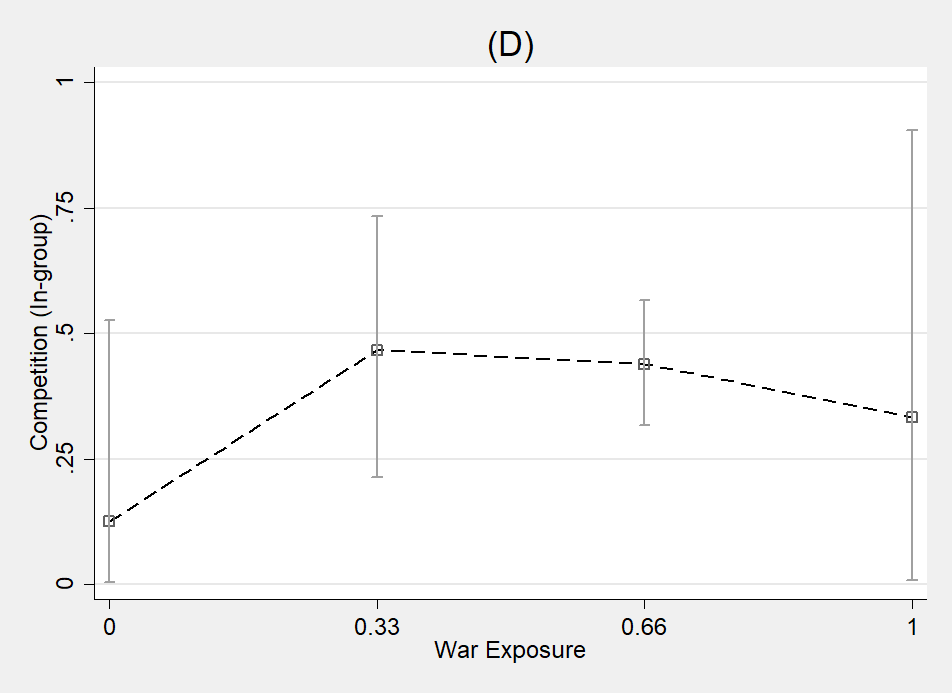
\includegraphics[width=0.8\linewidth]{"chapters/slfootball/figures/f4_we_competition.eps"}
  \caption{Foul cards, competitiveness and exposure to violence}
  \label{fig:slf:we_competition}
  \subcaption*{\textit{Notes:} Competition and war expose: Panel A: Foul Card and war exposure for the entire sample; Panel B: willingness to compete and war exposure, entire sample; Panel C: willingness to compete and war exposure,  out-group only; Panel D: willingness to compete and war exposure, in-group only. All panels show binomial confidence intervals at the 95\% level.}
  \end{center}
\end{figure}

We find that war exposure results in out-group competition. At the median of all covariates, subjects most exposed to conflict-related violence are 51\% more likely to join a competition against the out-group, significant at $\alpha$ = 0.05 (Table \ref{tab:slf:compete}, columns 1-2).\footnote{The coefficient on exposure to war-related violence increases when observable controls are included. Following \citet{Bellows2009b}, this suggests that omitted bias is unlikely to explain away the effect \citep[see also][]{Altonji2005}.} On the other hand we cannot reject the null of no effect for in-group competitive behavior (Table \ref{tab:slf:compete}, columns 3-4), as well as across groups (Table \ref{tab:slf:compete}, column 5).\footnote{The coefficient on the group interaction term is large and negative, as expected. This is suggestive of a substantial though not significant difference in coefficients across groups. As a further test, we allow for different residual variation across groups and compute Allison’s delta (-0.570)--the effect of conflict exposure on competition can thus be interpreted as being 57\% smaller towards the in-group than towards the out-group \citep{Allison1999a}}

\begin{table}[p!]
\centering
\begin{threeparttable}[p!]
	\caption{Willingness to Compete}
	\label{tab:slf:compete}
	\singlespacing
	%\renewcommand{\arraystretch}{0.6}
	% \tiny 
	% \scriptsize
	%\footnotesize
	\small
	% \normalsize
	{
\def\sym#1{\ifmmode^{#1}\else\(^{#1}\)\fi}
\begin{tabular}{l*{5}{c}}
\hline\hline
                    &\multicolumn{1}{c}{(1)}&\multicolumn{1}{c}{(2)}&\multicolumn{1}{c}{(3)}&\multicolumn{1}{c}{(4)}&\multicolumn{1}{c}{(5)}\\
                    &\multicolumn{1}{c}{Out-group}&\multicolumn{1}{c}{Out-group}&\multicolumn{1}{c}{In-group}&\multicolumn{1}{c}{In-group}&\multicolumn{1}{c}{Pooled}\\
\hline
Self-select in tournament&                     &                     &                     &                     &                     \\
War Exposure        &       0.485\sym{**} &       0.623\sym{**} &       0.274         &     -0.0218         &       0.499\sym{**} \\
                    &     (0.222)         &     (0.248)         &     (0.227)         &     (0.256)         &     (0.233)         \\
[1em]
Ingroup (d)         &                     &                     &                     &                     &       0.304         \\
                    &                     &                     &                     &                     &     (0.198)         \\
[1em]
Exposure to conflict × in-group&                     &                     &                     &                     &      -0.559\sym{*}  \\
                    &                     &                     &                     &                     &     (0.338)         \\
[1em]
ind\_age==20-24 (d)  &                     &     -0.0489         &                     &     -0.0928         &      -0.106         \\
                    &                     &     (0.172)         &                     &     (0.131)         &     (0.100)         \\
[1em]
ind\_age==25-29 (d)  &                     &     -0.0374         &                     &                     &      0.0979         \\
                    &                     &     (0.262)         &                     &                     &     (0.208)         \\
[1em]
ind\_age==30-34      &                     &                     &                     &                     &                     \\
                    &                     &                     &                     &                     &                     \\
[1em]
ind\_edu             &                     &       0.258\sym{**} &                     &      0.0652         &       0.156\sym{*}  \\
                    &                     &     (0.126)         &                     &     (0.122)         &    (0.0869)         \\
[1em]
Meals per day       &                     &      -0.104         &                     &      -0.151         &      -0.136\sym{*}  \\
                    &                     &     (0.128)         &                     &    (0.0981)         &    (0.0741)         \\
[1em]
Muslim (d)          &                     &       0.231         &                     &     -0.0334         &      0.0376         \\
                    &                     &     (0.148)         &                     &     (0.178)         &     (0.117)         \\
[1em]
ind\_mende (d)       &                     &     -0.0771         &                     &      0.0301         &    -0.00607         \\
                    &                     &     (0.148)         &                     &     (0.130)         &    (0.0944)         \\
[1em]
Played whole game (d)&                     &       0.278\sym{*}  &                     &       0.117         &       0.168\sym{*}  \\
                    &                     &     (0.159)         &                     &     (0.122)         &    (0.0926)         \\
[1em]
Self-declared skills&                     &       0.103         &                     &      -0.168         &     -0.0145         \\
                    &                     &     (0.285)         &                     &     (0.302)         &     (0.206)         \\
[1em]
Scored (d)          &                     &      -0.280\sym{*}  &                     &      -0.196         &      -0.202\sym{*}  \\
                    &                     &     (0.159)         &                     &     (0.140)         &     (0.109)         \\
[1em]
Won the football game (d)&                     &      0.0965         &                     &      0.0116         &      0.0333         \\
                    &                     &     (0.139)         &                     &     (0.124)         &    (0.0923)         \\
[1em]
Left footed (d)     &                     &      -0.243\sym{*}  &                     &      -0.233\sym{*}  &      -0.224\sym{**} \\
                    &                     &     (0.136)         &                     &     (0.129)         &    (0.0957)         \\
\hline
N                   &          70         &          61         &          92         &          78         &         141         \\
Pseudo R-Squared    &       0.055         &       0.171         &       0.011         &       0.065         &       0.087         \\
\hline\hline
\end{tabular}
}

	\begin{tablenotes}
		\footnotesize
		\item \textit{Notes:} robit marginal effects. Column 1 reports the univariate marginal effect of exposure to conflict on our experimental measure of willingness to compete towards the out-group (see Appendix I for variable definitions). Column 2 adds individual and football game related controls. Column 3 reports the univariate marginal effect of exposure to conflict on our experimental measure of willingness to compete towards the in-group. Column 4 adds individual and football game related controls. Column 5 reports the pooled marginal effect of exposure to conflict our experimental measure of willingness to compete, including individual and football game related controls, a group dummy, and an interaction term. Robust standard errors in parentheses. * p $<$ 0.10, ** p $<$ 0.05, *** p $<$ 0.01.
		\item
	\end{tablenotes}
\end{threeparttable}
\end{table}


To probe the robustness of this result we run several additional analyses. As mentioned in the previous section, our results may be driven by age. In Table \ref{tab:slf:compete}, column 2 we control for age and age squared. In Appendix Table \ref{tab:slf:compete_fe} we run a more flexible specification of the regression—adding age and age-group fixed effects. The coefficient of conflict exposure remains stable and robustly significant. Next, we assess whether selective migration drives our result. In Appendix Table \ref{tab:slf:compete_migrate} we separate participants that never moved out of Kenema district from those who did. The coefficient on the two separate groups is stable (Table \ref{tab:slf:compete_migrate}, columns 1-2), and the interaction term insignificant (Table \ref{tab:slf:compete_migrate}, columns 3-4).\footnote{Note that due to the small sample size measurement error inflates standard errors.}  This attenuates the concern that our results are due to selective migration patterns. In addition, our results are robust to the introduction of forced displacement as an additional source of war-related trauma, as well as football-match fixed effects, team fixed effects and clustering standard errors at the football team level (see Appendix Table \ref{tab:slf:compete_disp}). Finally, while we control for proxies of proxies of sportive ability throughout (i.e. playing the whole football game and self-declared skills), willingness to compete may also be a function of risk preferences, expected relative performance in the effort game, and actual skills. Our result holds to introducing these controls both separately and jointly – and the coefficients maintain relative constancy (see Appendix Table \ref{tab:slf:compete_abl}).

\section{Discussion and conclusion}
\label{sec:slf:discussion}
We explore whether exposure to war-related violence affects the competitiveness of youth participating in a local street football tournament and a series of lab-in-field experiments in Sierra Leone. Previous economic literature on the consequences of civil war on preferences documents increases in-group cooperation, political activeness and altruism. The main contribution of this study is to provide insight into the determinants of competitive behavior and its relation with exposure to violent conflict. We bring new evidence that increased parochial altruism is a two-fold process—increasing in-group cooperation while exacerbating out-group antagonism. 

Increased antagonism matters for post-conflict development as it shapes aggressiveness and, perhaps more saliently, competitiveness. To study war induced out-group dynamics we look both at aggressiveness during a football game and competitive behavior in laboratory experiment. We find that subjects more exposed to war violence during early childhood and preadolescence are not only robustly more likely to commit fouls during a football game, but are also more likely to self-select into a competition against an out-group in our experiment. Civil war does not only seem to foster cooperation towards perceived in-groups, but curbs distaste for free competition against perceived out-groups. Being more prone to cooperate and engage in public debates affects the community level provision of public goods, potentially promoting economic development \citep{Bellows2009b}. Similarly, accepting inequality-averse outcomes driven by a fair and regulated competition is a fundamental element of economic growth \citep{Bartling2009b}.
 
Our findings are tentative; different types of conflicts could have varying legacies, and the human cost of conflict may never be justified by its ``externalities'' \citep{CassarAlessandra}. Yet, a growing body of evidence about war violence victims’ profound changes in individual beliefs, values, and preferences poses new challenges to policy makers and post-conflict recovery strategists. It rejects the notion of conflict as ``development in reverse'' \cite{Collier2003}. Not only has war historically promoted state formation and nation building – ultimately strengthening institutional capacity \citep{Tilly1975} -- it may also be at the core of inclusive and dynamic societal transformations. Policy makers responsible for post-war recovery should be aware of the extent of these transformations and recognize heterogeneity among communities and individuals, not overlooking the significance of autonomous responses.


\clearpage
\section{Appendix I: Variable Definitions}
%\addcontentsline{toc}{section}{Appendix I: Variable Definitions}

\textit{Exposure to Conflict.} An individual victimization index resulting from the average response to these violence related questions: ``during war time...'' ``did you ever witness combat, shooting and explosions?'', ``did you ever see a person injured because of war-related violence?'' and ``did you personally suffer from physical injury because of war-related violence?''.

\textit{Parents Fought in War.} Individual level dummy variable taking value of unity if any one of parents of respondent $i$ have been active belligerents during the civil conflict, regardless of combatting sides.
\textit{Age.} Age of respondent $i$ as measured in years, rounded down to the age at the last birthday.

\textit{Education Level.} Individual level variable taking value 1 if the respondent was currently in primary school, 2 if the respondent was currently in junior secondary school, 3 if the respondent was currently in senior secondary school, 4 if respondent was enrolled or had completed tertiary education.

\textit{Mende (Fula, Mandingo, Temne) Tribe.} Individual level dummy taking value of unity if the $i$-th respondent self-declared to be ethically Mende (Fula, Mandingo, Temne), zero if else.


\textit{Muslim Religion.} Individual level dummy taking value of unity if the $i$-th respondent self-declared to be Muslim by religion, zero if else.

\textit{Meals per Day.} Household level index representing the self-reported full meal consumtion patterns of respondent $i$’s household.

\textit{Always in Kenema.} Individual level dummy variable taking value of unity if the i-th respondent never left Kenema district over the course of the war.

\textit{Left Footed.} Individual level dummy variable taking value of unity if the $i$-th respondent self-declared to be predominantly left-footed, zero if else.

\textit{Played Whole Game.} Individual level dummy variable taking value of unity if the $i$-th respondent had respondent positively to the question ``did you play the whole football game?'', zero if else. The answer was crosschecked with the control questions ``how many minutes did you play in this game'' and ``How many minutes did the game last in total?''; the dummy would take a value of zero if the ratio of their responses differed from unity.

\textit{Self-declared Skills.} Individual level index constructed as the answer to the question ``Compared to your team mates, how skillful would you say you are?''; on a scale of 1 (least skilled) to 5 (most skilled), standardized between 0 and 1. 

\textit{Scored.} Individual level dummy variable taking value of unity if the $i$-th respondent had scored at least one goal during the football game, zero if else.

\textit{Won the Football Game.} Team level dummy variable taking value of 1 if the team of respondent $i$ has won the football game, zero if else. Out of 14 games 1 ended up in a draw and the penalty kicks were postponed to the next day due to insufficient light.

\textit{Foul Card in Football Game.} Individual level dummy variable taking value of unity if the $i$-th respondent had received at least one yellow/red card up to that stage of the tournament.

\textit{Risk Propensity.} Individual level variable based on the respondents’ six choices in the risk game, spanning from zero (i.e. never gamble) to one (i.e. always gamble), and allowing for indifference by taking the last switch point as significant. The index is standardized.

\textit{Sharing in Dictator Game.} The value donated in the relevant dictator game (standardized).

\textit{Expected Relative Performance.} Individual level index constructed as the answer to the question ``Compared to the rest of today’s players, how well do you think you will perform in this game?''; on a scale of 0 (the worst) to 5 (the best), standardized between 0 and 1. 

\textit{Balls on Target.} The number of balls shot by the $i$-th subject in the effort game, successfully entering the basket (out of 10).
\clearpage

\section{Appendix II: Sensitivity Analysis}
%\addcontentsline{toc}{section}{Appendix II: Sensitivity Analysis}
\setcounter{table}{0}
\renewcommand{\thetable}{\arabic{chapter}.A\arabic{table}}

\begin{center}
\begin{threeparttable}[p!]
	\caption{Willingness to Compete (out-group)}
	\label{tab:slf:compete_fe}
	\singlespacing
	%\renewcommand{\arraystretch}{0.6}
	% \tiny 
	% \scriptsize
	%\footnotesize
	\small
	% \normalsize
	{
\def\sym#1{\ifmmode^{#1}\else\(^{#1}\)\fi}
\begin{tabular}{l*{4}{c}}
\hline\hline
                    &\multicolumn{1}{c}{(1)}&\multicolumn{1}{c}{(2)}&\multicolumn{1}{c}{(3)}&\multicolumn{1}{c}{(4)}\\
                    &\multicolumn{1}{c}{\specialcell{1-year\\age-group f.e.}}&\multicolumn{1}{c}{\specialcell{2-year\\age-group f.e.}}&\multicolumn{1}{c}{\specialcell{3-year\\age-group f.e.}}&\multicolumn{1}{c}{\specialcell{4-year\\age-group f.e.}}\\
\hline
Self-select in tournament&                     &                     &                     &                     \\
War Exposure        &       0.693\sym{*}  &       0.520\sym{**} &       0.524\sym{**} &       0.470\sym{**} \\
                    &     (0.367)         &     (0.239)         &     (0.230)         &     (0.233)         \\
[1em]
Education Level     &       0.383\sym{**} &       0.250\sym{**} &       0.223\sym{**} &       0.178\sym{*}  \\
                    &     (0.153)         &    (0.0991)         &    (0.0916)         &    (0.0961)         \\
[1em]
Meals per day       &     -0.0176         &      0.0397         &      0.0179         &     -0.0111         \\
                    &     (0.156)         &     (0.110)         &     (0.115)         &     (0.110)         \\
[1em]
Muslim (d)          &       0.582\sym{***}&       0.408\sym{***}&       0.325\sym{***}&       0.323\sym{***}\\
                    &     (0.108)         &    (0.0929)         &     (0.116)         &     (0.118)         \\
[1em]
Mende (d)           &     0.00397         &     -0.0666         &      -0.121         &      -0.114         \\
                    &     (0.196)         &     (0.149)         &     (0.143)         &     (0.147)         \\
[1em]
Played whole game (d)&       0.642\sym{***}&       0.445\sym{***}&       0.494\sym{***}&       0.431\sym{***}\\
                    &     (0.166)         &     (0.138)         &     (0.132)         &     (0.136)         \\
[1em]
Self-declared skills&      -0.285         &    -0.00472         &      0.0568         &      0.0178         \\
                    &     (0.316)         &     (0.257)         &     (0.272)         &     (0.254)         \\
[1em]
Scored (d)          &      -0.502\sym{***}&      -0.302\sym{**} &      -0.370\sym{***}&      -0.250         \\
                    &     (0.102)         &     (0.123)         &     (0.102)         &     (0.152)         \\
[1em]
Won the football game (d)&       0.307         &       0.167         &      0.0849         &       0.106         \\
                    &     (0.188)         &     (0.142)         &     (0.139)         &     (0.140)         \\
[1em]
Left footed (d)     &      -0.113         &     -0.0498         &      -0.125         &      -0.151         \\
                    &     (0.219)         &     (0.147)         &     (0.158)         &     (0.142)         \\
[1em]
Constant            &                     &                     &                     &                     \\
                    &                     &                     &                     &                     \\
\hline
N                   &          56         &          65         &          69         &          69         \\
R2                  &       0.412         &       0.309         &       0.256         &       0.229         \\
\hline\hline
\end{tabular}
}

	\begin{tablenotes}
		\footnotesize
		\item \textit{Notes:} Probit marginal effects. Column 1 reports the marginal effect of exposure to conflict on our experimental measure of willingness to compete towards the out-group (see Appendix I for variable definitions), including individual and football game related controls, as well as 1-year age fixed effects. Column 2 replaces 1-year age fixed effects with 2-year age fixed effects. Column 3 replaces 2-year age fixed effects with 3-year age fixed effects. Column 4 replaces 3-year age fixed effects with 4-year age fixed effects. 14 observations dropped in (1), 5 observations dropped in (2) and 1 observation dropped in (3), due to quasi-separation issues related to small group fixed effects. Robust standard errors in parentheses. * p $<$ 0.10, ** p $<$ 0.05, *** p $<$ 0.01.
		\item
	\end{tablenotes}
\end{threeparttable}
\end{center}

\pagebreak

\begin{center}
\begin{threeparttable}[p!]
	\caption{Willingness to Compete (out-group)}
	\label{tab:slf:compete_migrate}
	\singlespacing
	%\renewcommand{\arraystretch}{0.6}
	% \tiny 
	% \scriptsize
	\footnotesize
	%\small
	% \normalsize
	{
\def\sym#1{\ifmmode^{#1}\else\(^{#1}\)\fi}
\begin{tabular}{l*{4}{c}}
\hline\hline
                    &\multicolumn{1}{c}{(1)}&\multicolumn{1}{c}{(2)}&\multicolumn{1}{c}{(3)}&\multicolumn{1}{c}{(4)}\\
                    &\multicolumn{1}{c}{\specialcell{Outgroup:\\Always in\\Kenema}}&\multicolumn{1}{c}{\specialcell{Outgroup:\\Migrated}}&\multicolumn{1}{c}{\specialcell{Outgroup:\\All}}&\multicolumn{1}{c}{\specialcell{Pooled}}\\
\hline
                    &                     &                     &                     &                     \\
Exposure to conflict&       0.755         &       0.622         &       0.553\sym{**} &       0.621\sym{**} \\
                    &     (0.497)         &     (0.430)         &     (0.282)         &     (0.259)         \\
[1em]
Always in Kenema (d)&                     &                     &      -0.350         &     -0.0550         \\
                    &                     &                     &     (0.325)         &     (0.207)         \\
[1em]
Exposure to conflict x Always in Kenema&                     &                     &       0.214         &      -0.217         \\
                    &                     &                     &     (0.506)         &     (0.327)         \\
[1em]
Ingroup (d)         &                     &                     &                     &       0.139         \\
                    &                     &                     &                     &     (0.197)         \\
[1em]
Exposure to conflict × in-group&                     &                     &                     &      -0.278         \\
                    &                     &                     &                     &     (0.314)         \\
[1em]
Age                 &      -0.263         &       1.217\sym{**} &    -0.00285         &      -0.135         \\
                    &     (0.303)         &     (0.491)         &     (0.210)         &     (0.119)         \\
[1em]
Age squared         &     0.00686         &     -0.0277\sym{**} &    0.000747         &     0.00335         \\
                    &   (0.00754)         &    (0.0111)         &   (0.00474)         &   (0.00269)         \\
[1em]
Education Level     &       0.181         &      0.0646         &       0.167         &       0.138\sym{**} \\
                    &     (0.116)         &     (0.185)         &     (0.103)         &    (0.0633)         \\
[1em]
Meals per day       &     -0.0832         &      0.0506         &     -0.0539         &     -0.0730         \\
                    &     (0.135)         &     (0.243)         &     (0.126)         &    (0.0732)         \\
[1em]
Muslim (d)          &       0.276\sym{**} &     -0.0751         &       0.286\sym{**} &      0.0105         \\
                    &     (0.120)         &     (0.248)         &     (0.122)         &     (0.103)         \\
[1em]
Mende (d)           &      -0.179         &      -0.109         &      -0.157         &     -0.0324         \\
                    &     (0.226)         &     (0.271)         &     (0.153)         &    (0.0900)         \\
[1em]
Played whole game (d)&       0.212         &       0.602\sym{***}&       0.395\sym{***}&       0.220\sym{**} \\
                    &     (0.173)         &     (0.191)         &     (0.143)         &    (0.0857)         \\
[1em]
Self-declared skills&     -0.0845         &    -0.00360         &     -0.0436         &     -0.0690         \\
                    &     (0.347)         &     (0.406)         &     (0.263)         &     (0.193)         \\
[1em]
Scored (d)          &      -0.134         &      -0.409         &      -0.277\sym{*}  &      -0.136         \\
                    &     (0.183)         &     (0.454)         &     (0.155)         &     (0.110)         \\
[1em]
Won the football game (d)&      0.0281         &       0.391\sym{*}  &       0.161         &      0.0139         \\
                    &     (0.169)         &     (0.222)         &     (0.142)         &    (0.0860)         \\
[1em]
Left footed (d)     &      -0.250\sym{**} &      -0.159         &      -0.184         &      -0.219\sym{**} \\
                    &     (0.112)         &     (0.400)         &     (0.142)         &    (0.0875)         \\
\hline
N                   &          36         &          34         &          70         &         162         \\
R2                  &        0.30         &        0.33         &        0.23         &        0.13         \\
\hline\hline
\end{tabular}
}

	\begin{tablenotes}
		\footnotesize
		\item \textit{Notes:} Probit marginal effects. Column 1 reports the marginal effect of exposure to conflict on our experimental measure of willingness to compete towards the out-group (see Appendix I for variable definitions), including individual and football game related controls, for the subsample of respondents who were born and had never moved out of Kenema district. Column 2 presents the outcomes for the remaining subsample, born elsewhere or temporarily out-migrated from Kenema district during the conflict. Column 3 reports the marginal effect of exposure to conflict on our experimental measure of willingness to compete towards the out-group, including individual and football game related controls, and a variable capturing the absence of temporary out-migration. Column 4 presents the outcome for the pooled sample (in-group and out-group). Robust standard errors in parentheses. * p $<$ 0.10, ** p $<$ 0.05, *** p $<$ 0.01.
		\item
	\end{tablenotes}
\end{threeparttable}
\end{center}

\pagebreak

\begin{center}
\begin{threeparttable}[p!]
	\caption{Willingness to Compete (out-group)}
	\label{tab:slf:compete_disp}
	\singlespacing
	%\renewcommand{\arraystretch}{0.6}
	% \tiny 
	% \scriptsize
	%\footnotesize
	\small
	% \normalsize
	{
\def\sym#1{\ifmmode^{#1}\else\(^{#1}\)\fi}
\begin{tabular}{l*{4}{c}}
\hline\hline
                    &\multicolumn{1}{c}{(1)}&\multicolumn{1}{c}{(2)}&\multicolumn{1}{c}{(3)}&\multicolumn{1}{c}{(4)}\\
                    &\multicolumn{1}{c}{Self-select in tournament}&\multicolumn{1}{c}{Self-select in tournament}&\multicolumn{1}{c}{Self-select in tournament}&\multicolumn{1}{c}{Self-select in tournament}\\
\hline
Self-select in tournament&                     &                     &                     &                     \\
War Exp. incl. displacement&       0.916\sym{***}&                     &                     &                     \\
                    &     (0.339)         &                     &                     &                     \\
[1em]
Exposure to conflict&                     &       0.882\sym{**} &       0.974\sym{**} &       0.690\sym{**} \\
                    &                     &     (0.392)         &     (0.447)         &     (0.322)         \\
[1em]
ind\_age==20-24 (d)  &       0.049         &       0.080         &       0.221         &       0.086         \\
                    &     (0.212)         &     (0.248)         &     (0.283)         &     (0.212)         \\
[1em]
ind\_age==25-29      &                     &                     &                     &                     \\
                    &                     &                     &                     &                     \\
[1em]
ind\_edu             &       0.191         &       0.062         &      -0.069         &       0.205         \\
                    &     (0.150)         &     (0.173)         &     (0.207)         &     (0.128)         \\
[1em]
Meals per day       &      -0.074         &       0.132         &       0.370         &      -0.031         \\
                    &     (0.154)         &     (0.205)         &     (0.238)         &     (0.115)         \\
[1em]
Muslim (d)          &       0.501\sym{***}&                     &                     &       0.495\sym{***}\\
                    &     (0.088)         &                     &                     &     (0.073)         \\
[1em]
ind\_mende (d)       &      -0.251         &      -0.412         &      -0.397         &      -0.210         \\
                    &     (0.186)         &     (0.256)         &     (0.276)         &     (0.169)         \\
[1em]
Played whole game (d)&       0.396\sym{**} &       0.554\sym{**} &       0.660\sym{***}&       0.422\sym{***}\\
                    &     (0.183)         &     (0.217)         &     (0.236)         &     (0.105)         \\
[1em]
Self-declared skills&       0.278         &       0.257         &      -0.026         &       0.226         \\
                    &     (0.339)         &     (0.366)         &     (0.442)         &     (0.327)         \\
[1em]
Scored (d)          &      -0.421\sym{***}&      -0.247         &      -0.010         &      -0.393\sym{***}\\
                    &     (0.144)         &     (0.266)         &     (0.408)         &     (0.147)         \\
[1em]
Won the football game (d)&       0.383\sym{**} &       0.382\sym{**} &                     &       0.328\sym{**} \\
                    &     (0.159)         &     (0.166)         &                     &     (0.161)         \\
[1em]
Left footed (d)     &      -0.326\sym{**} &      -0.413\sym{***}&      -0.500\sym{***}&      -0.300\sym{**} \\
                    &     (0.142)         &     (0.154)         &     (0.107)         &     (0.135)         \\
[1em]
Constant            &                     &                     &                     &                     \\
                    &                     &                     &                     &                     \\
\hline
N                   &          49         &          40         &          35         &          49         \\
R2                  &       0.264         &       0.289         &       0.296         &       0.253         \\
\hline\hline
\multicolumn{5}{l}{\footnotesize Marginal effects; Standard errors in parentheses}\\
\multicolumn{5}{l}{\footnotesize  (d) for discrete change of dummy variable from 0 to 1}\\
\multicolumn{5}{l}{\footnotesize \sym{*} \(p<0.10\), \sym{**} \(p<0.05\), \sym{***} \(p<0.01\)}\\
\end{tabular}
}

	\begin{tablenotes}
		\footnotesize
		\item \textit{Notes:} Probit marginal effects. Column 1 reports the marginal effect of exposure to conflict on our experimental measure of willingness to compete towards the out-group (see Appendix I for variable definitions), including individual and football game related controls, were the exposure to conflict includes a dummy for forced displacement as additional measure of victimization. Column 2 includes football match fixed effects. Column 3 includes team fixed effects. Column 4 clusters standard errors at the team level. 7 Observations dropped in (3) due to quasi-separation issues related to small group fixed effects. Robust standard errors in parentheses. * p $<$ 0.10, ** p $<$ 0.05, *** p $<$ 0.01.
		\item
	\end{tablenotes}
\end{threeparttable}
\end{center}

\pagebreak

\begin{center}
\begin{threeparttable}[p!]
	\caption{Willingness to Compete (out-group)}
	\label{tab:slf:compete_abl}
	\singlespacing
	%\renewcommand{\arraystretch}{0.6}
	% \tiny 
	% \scriptsize
	%\footnotesize
	\small
	% \normalsize
	{
\def\sym#1{\ifmmode^{#1}\else\(^{#1}\)\fi}
\begin{tabularx}{\textwidth}{Xl*{4}{c}}
\hline\hline
                    &\multicolumn{1}{c}{(1)}&\multicolumn{1}{c}{(2)}&\multicolumn{1}{c}{(3)}&\multicolumn{1}{c}{(4)}\\
                    &\multicolumn{1}{c}{\specialcell{Risk\\Preferences}}&\multicolumn{1}{c}{\specialcell{Expected Relative\\Performance}}&\multicolumn{1}{c}{\specialcell{Actual\\Performance}}&\multicolumn{1}{c}{\specialcell{Risk, Expected, and\\Actual Performance}}\\
\hline
                    &                     &                     &                     &                     \\
Exposure to conflict&       0.516\sym{**} &       0.535\sym{**} &       0.470\sym{*}  &       0.495\sym{*}  \\
                    &     (0.243)         &     (0.250)         &     (0.253)         &     (0.256)         \\
[1em]
Risk Preferences    &      0.0262         &                     &                     &      0.0179         \\
                    &    (0.0723)         &                     &                     &    (0.0715)         \\
[1em]
Expected performance&                     &       0.489         &                     &       0.467         \\
                    &                     &     (0.580)         &                     &     (0.591)         \\
[1em]
Balls on target     &                     &                     &     -0.0230         &     -0.0233         \\
                    &                     &                     &    (0.0386)         &    (0.0396)         \\
[1em]
Age                 &      0.0992         &      0.0872         &      0.0889         &      0.0699         \\
                    &     (0.185)         &     (0.186)         &     (0.183)         &     (0.188)         \\
[1em]
Age squared         &    -0.00145         &    -0.00126         &    -0.00117         &   -0.000842         \\
                    &   (0.00420)         &   (0.00421)         &   (0.00417)         &   (0.00427)         \\
[1em]
Education Level     &       0.172\sym{*}  &       0.159         &       0.180\sym{*}  &       0.169         \\
                    &    (0.0988)         &     (0.101)         &     (0.101)         &     (0.104)         \\
[1em]
Meals per day       &     -0.0191         &     -0.0299         &     -0.0198         &     -0.0318         \\
                    &     (0.111)         &     (0.109)         &     (0.110)         &     (0.111)         \\
[1em]
Muslim (d)          &       0.306\sym{**} &       0.311\sym{***}&       0.315\sym{***}&       0.320\sym{***}\\
                    &     (0.119)         &     (0.118)         &     (0.117)         &     (0.117)         \\
[1em]
Mende (d)           &     -0.0966         &     -0.0740         &     -0.0828         &     -0.0821         \\
                    &     (0.147)         &     (0.152)         &     (0.149)         &     (0.150)         \\
[1em]
Played whole game (d)&       0.403\sym{***}&       0.373\sym{**} &       0.429\sym{***}&       0.397\sym{***}\\
                    &     (0.138)         &     (0.146)         &     (0.140)         &     (0.151)         \\
[1em]
Self-declared skills&      0.0257         &     -0.0621         &      0.0430         &     -0.0318         \\
                    &     (0.256)         &     (0.275)         &     (0.261)         &     (0.283)         \\
[1em]
Scored (d)          &      -0.268\sym{*}  &      -0.253         &      -0.288\sym{**} &      -0.277\sym{*}  \\
                    &     (0.148)         &     (0.155)         &     (0.141)         &     (0.146)         \\
[1em]
Won the football game (d)&       0.131         &       0.114         &       0.146         &       0.143         \\
                    &     (0.137)         &     (0.134)         &     (0.141)         &     (0.143)         \\
[1em]
Left footed (d)     &      -0.187         &      -0.156         &      -0.212         &      -0.199         \\
                    &     (0.140)         &     (0.150)         &     (0.143)         &     (0.150)         \\
\hline
N                   &          70         &          70         &          70         &          70         \\
R2                  &       0.209         &       0.215         &       0.211         &       0.219         \\
\hline\hline
\end{tabularx}
}

	\begin{tablenotes}
		\footnotesize
		\item \textit{Notes:} Probit marginal effects. Column 1 reports the marginal effect of exposure to conflict on our experimental measure of willingness to compete towards the out-group (see Appendix I for variable definitions), including individual and football game related controls, and our experimental measure of risk preferences. Column 2 includes expected relative performance, standardized between 0 (the worst) and 1 (the best). Column 3 includes actual performance in terms of the number of balls on target (standardized). Column 4 includes all three measures risk preferences, performance expectation, and skills. Robust standard errors in parentheses.  * p $<$ 0.10, ** p $<$ 0.05, *** p $<$ 0.01.
		\item
	\end{tablenotes}
\end{threeparttable}
\end{center}

\clearpage
\bibliographystyle{chicago}
%path to .bib file (e.g. automatically exported by mendeley) DO NOT include the file extension!
\bibliography{tex_helpers/Thesis}